\section{Approaches}

Before starting the actual implementation process, we first thought about different
ways in which the Lanczos algorithm could be realized in the Apache Flink system. We
identified three different approaches that we could take. One of them would be to
leverage Flink's delta iteration construction, another one would be to make use of
Mahout's implementation of the Lanczos algorithm for the Hadoop framework. The third
possibility we found is to still implement the actual algorithm manually in Flink, but
without using delta iterations to model the algorithm's iterative nature.

\subsection{Using Flink Delta Iterations}

% Delta Iterations
% - Why DELTA iterations?
%    --> Briefly explain delta iterations
%    --> Current iteration has small input that results from previous iteration (= work set)
%    --> Result of every iteration is appended to final result (= result set)

While planning the implementation part of our project, we consulted both the official
Flink 0.8 documentation [1] as well as the Flink community directly (mainly through
the \#flink IRC channel in the Freenode IRC network) in order to find reasonable
approaches for our intent. The first and most obvious approach both of these sources 
pointed to was to take advantage of Flink's delta iteration capabilities. But what
exactly are delta iterations, how do they compare to standard Flink iterations and why 
would we choose the former over the latter?

% - Flink provides an iteration operator specifically for the purpose of implementing iterative algorithm
%    --> Idiomatic way
%    --> Two variants: Iterate + Delta Iterate
%        --> For both: Define step function that will be invoked repeatedly until termination condition is reached
%        --> Iterate:
%            - For simple iterations
%            - Step function takes entire input and computes next version of partial solution
%            - Final result = partial solution of the last iteration
%        --> Delta Iterate:
%            - Specifically designed for incremental iterations (= iterations that only modify small parts
%              of their solution in every iteration and by that evolve the solution instead of fully recomputing it
%              in every iteration)
%                --> More effective, because each iteration operates only on small subset of data
%            - Each step...
%                ...takes current work set and produces new work set
%                ...updates part of the solution set
%            - Final result = solution set after last iteration

Flink provides an iteration operator specifically for the purpose of implementing
iterative algorithms, as these kinds of algorithms occur in many domains of data
analysis and as the general interest in running them on huge data sets is increasing.
The mere existence of this special kind of operator (and the fact that we were explicitly
pointed to it by the Flink community) led us to the conclusion that this must be the
idiomatic way of implementing the Lanczos algorithm in Flink. Two variants of the
iteration operator are provided by Flink: \textbf{Iterate} (we will also call this the
standard iteration) and \textbf{Delta Iterate}. The general idea of both of these operators
is that the programmer defines a step function that will be invoked repeatedly on the
current state of the data until a specified termination condition is reached. [1]

% TODO: Are we allowed to use images from the Flink documentation?
\begin{figure}[h]
	\centering
	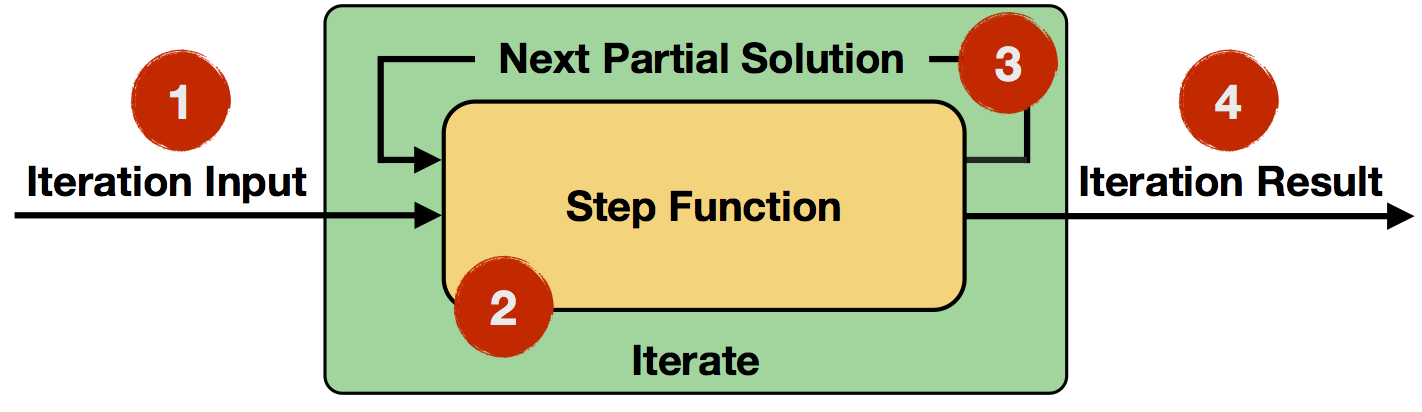
\includegraphics[width=0.8\textwidth]{images/iterations_iterate_operator}
	\caption{Graphical representation of the Iterate operator's data flow (source: 
	The Apache Software Foundation [1])}
	\label{fig:iterate_operator}
\end{figure}

Intended to be used for rather simple forms of iteration, the step function (2) of the 
\textbf{Iterate} operator pictured in figure \ref{fig:iterate_operator} always takes the 
entire input and computes the next partial solution from that (3). While the first step's input 
is the initial data set specified by the programmer (1), every step that follows consumes the 
partial solution produced by the preceding step. The Iterate operator's final result is simply 
the partial solution produced by the very last step (4). [1]

\begin{figure}[h]
	\centering
	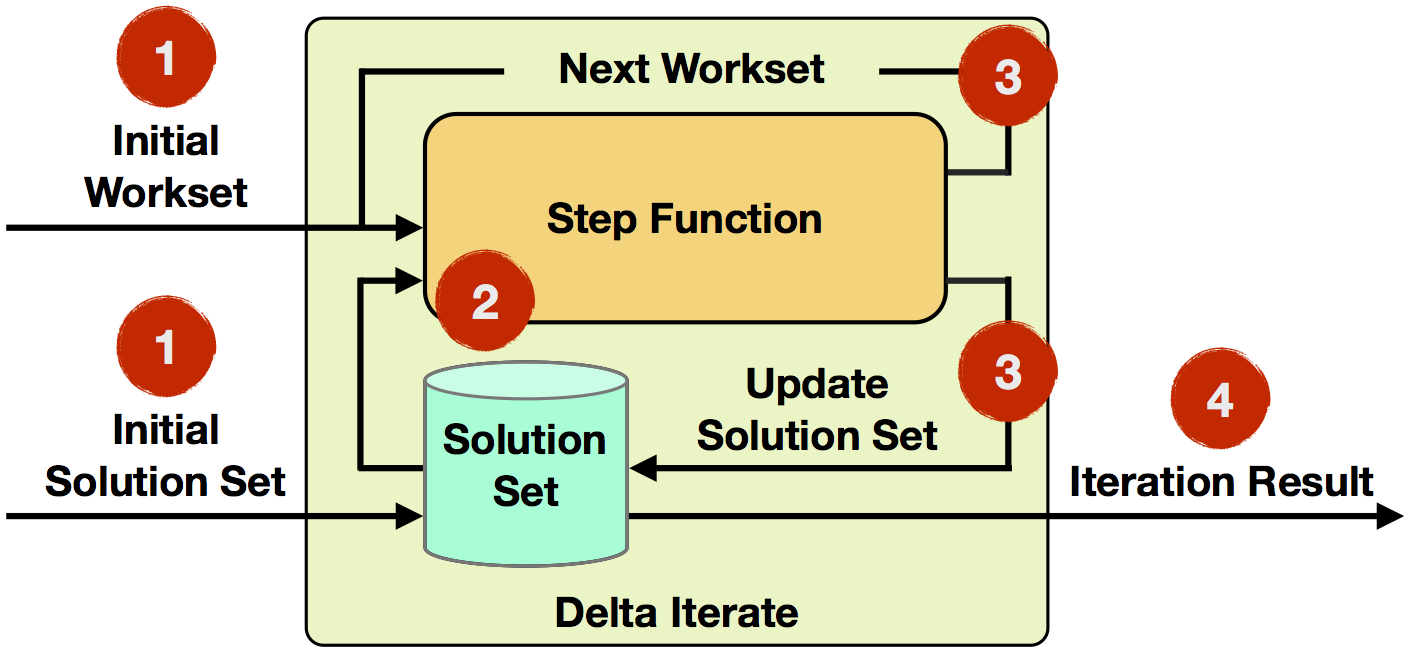
\includegraphics[width=0.8\textwidth]{images/iterations_delta_iterate_operator}
	\caption{Graphical representation of the Delta Iterate operator's data flow (source: 
	The Apache Software Foundation [1])}
	\label{fig:delta_iterate_operator}
\end{figure}

% - In every iteration of Lanczos algorithm...
%     ...only parts of the result of previous iteration are needed
%     ...only small parts are added to the final result
%     ...no existing parts of final result are modified
% ==> This matches intention of delta iterations perfectly

\subsection{Using Mahout's Lanczos Solver for Hadoop}

\subsection{Implementing an Iterative, Loop-based Construction}

% Mahout
% - Idea: Implement interface that Mahout's LanczosSolver uses 
%    --> don't actually implement lanczos in flink

% Iterative loop-based
%    --> Flink API/Optimizer doesn't know about iteration
%    --> Briefly explain Flink execution strategy/graph (Optimizer)